\documentclass[12pt,a4paper]{article}

\usepackage[utf8]{inputenc}
\usepackage[T1]{fontenc}
\usepackage{lmodern}
\usepackage[margin=2.5cm]{geometry}
\usepackage{graphicx}
\usepackage{booktabs}
\usepackage{float}
\usepackage{hyperref}
\usepackage{xcolor}
\usepackage{amsmath}
\usepackage{amssymb}
\usepackage{enumitem}
\usepackage{caption}
\usepackage{parskip}
\usepackage{fancyhdr}
\usepackage{setspace}
\usepackage{url}
\usepackage{tabularx}
\usepackage{placeins}
\usepackage{longtable}

\definecolor{covernavy}{HTML}{17324D}
\definecolor{coverblue}{HTML}{2C5E91}
\definecolor{covergold}{HTML}{C38C2D}
\definecolor{coverpanel}{HTML}{F3F6F9}

\hypersetup{
  colorlinks=true,
  linkcolor=blue!60!black,
  citecolor=blue!60!black,
  urlcolor=blue!70!black,
}

\setlength{\headheight}{13.6pt}
\addtolength{\topmargin}{-1.6pt}
\pagestyle{fancy}
\fancyhf{}
\fancyhead[L]{\small Technical Debt \& Hotspot Identification}
\fancyhead[R]{\small Vaibhav Sijaria --- 23BCI0063}
\fancyfoot[C]{\thepage}
\renewcommand{\headrulewidth}{0.4pt}

\setstretch{1.12}

\begin{document}

% ─── Title Page ───────────────────────────────────────────────────────────────
\pagenumbering{Alph}
\begin{titlepage}
\thispagestyle{empty}
\centering

\vspace*{0.25cm}

{\Large\bfseries\color{covernavy}VELLORE INSTITUTE OF TECHNOLOGY\par}
\vspace{0.15cm}
{\normalsize\color{coverblue}Software Engineering Case Study Report\par}
\vspace{0.28cm}
{\color{covergold}\rule{0.72\textwidth}{1.2pt}\par}

\vspace{0.5cm}

\includegraphics[width=3.15cm]{VIT_logo.png}

\vspace{0.55cm}
{\Large\bfseries\color{coverblue}Case Study No.\ 12\par}
\vspace{0.22cm}
{\LARGE\bfseries\color{covernavy}Technical Debt and Hotspot Identification\par}
\vspace{0.12cm}
{\large\color{coverblue}Complexity, Churn, and Code Smell Analysis\par}

\vspace{0.42cm}
\begin{minipage}{0.84\textwidth}
\centering
\color{black!75}
\normalsize
A comparative study of hotspot risk, bug-fix history, and remediation
priorities in \texttt{django/django} and
\texttt{huggingface/transformers}.
\end{minipage}

\vspace{0.7cm}
\makebox[\textwidth][c]{%
\fcolorbox{coverblue}{coverpanel}{%
\begin{minipage}[t]{0.62\textwidth}
\raggedright
\small
{\bfseries Course\par}
Software Engineering\par
\vspace{0.22cm}
{\bfseries Submitted By\par}
Vaibhav Sijaria\par
\vspace{0.22cm}
{\bfseries Registration No.\par}
23BCI0063\par
\vspace{0.22cm}
{\bfseries Submission Date\par}
6 April 2026\par
\vspace{0.22cm}
{\bfseries Focus\par}
Hotspot analysis using complexity, churn, and bug-fix history\par
\end{minipage}%
}%
}

\vfill

{\normalsize\color{covernavy}\bfseries School of Computer Science and Engineering (SCOPE)\par}

\end{titlepage}

\newpage
\pagenumbering{roman}
\tableofcontents
\newpage
\pagenumbering{arabic}

% ══════════════════════════════════════════════════════════════════════════════
\section{Aim}
\label{sec:aim}

The goal of this case study is to apply established technical-debt and hotspot-identification techniques to two prominent open-source Python repositories---\texttt{django/django} (a mature web framework) and \texttt{huggingface/transformers} (a fast-moving machine-learning library)---in order to rank their source files by defect risk, validate those rankings against historical bug-fix evidence, and propose a data-driven remediation plan.

Concretely, the study pursues three objectives:

\begin{enumerate}[leftmargin=2em]
  \item \textbf{Identify technical-debt hotspots} by combining static code complexity, commit-level churn, and code-smell indicators into a composite risk score for every non-test Python file.
  \item \textbf{Validate the rankings empirically} by testing whether the files flagged as high-risk do, in fact, accumulate more bug-fix commits over a two-year window.
  \item \textbf{Produce a prioritised remediation plan} that classifies the riskiest files into actionable categories (Refactor Now, Reduce Churn, Simplify, Monitor) with concrete recommendations.
\end{enumerate}

The scope is deliberately bounded: all data collection and analysis were carried out over a two-month lab-scale window using freely available tooling (see Section~\ref{sec:method}), making the approach reproducible by any team with access to a Git repository.

\subsection{Research Questions}
\label{sec:rq}

\begin{description}[style=unboxed,leftmargin=1em]
  \item[\textbf{RQ\,1.}] \emph{Which files in Django and Transformers carry the highest combined risk when cyclomatic complexity, code churn, and bug-fix frequency are considered together?}
  \item[\textbf{RQ\,2.}] \emph{Is there a statistically significant relationship between a file's hotspot score and its historical bug-fix activity?}
  \item[\textbf{RQ\,3.}] \emph{What concrete, prioritised refactoring actions can be recommended for the top-risk files in each project?}
\end{description}

% ══════════════════════════════════════════════════════════════════════════════
\section{Background Literature}
\label{sec:literature}

\subsection{Technical Debt}

Cunningham~[1] introduced the \emph{technical debt} metaphor in 1992 to describe how expedient but imperfect code decisions create an implicit cost that must be repaid through future refactoring.
Kruchten et al.~[7] later formalised a taxonomy that distinguishes \emph{code debt}, \emph{design debt}, \emph{testing debt}, and \emph{documentation debt}.
Fowler~[8] further distinguished between \emph{deliberate} and \emph{inadvertent} debt and between \emph{reckless} and \emph{prudent} debt, noting that even prudent decisions can accumulate debt over time.
This study focuses on \textbf{code-level debt}---files whose structural complexity and change patterns suggest elevated defect risk.

\subsection{Cyclomatic Complexity as a Risk Indicator}

McCabe~[2] proposed cyclomatic complexity (CCN) as a count of linearly independent paths through a function's control-flow graph.
Higher CCN implies more branches and, consequently, more potential for faults.
Empirical work by Basili and Perricone~[3] confirmed that modules with CCN~$>10$ are significantly more defect-prone, a threshold that remains widely cited.
We adopt the \texttt{lizard} static-analysis tool, which computes McCabe complexity for Python without requiring compilation.

\subsection{Code Churn and Defect Prediction}

Nagappan and Ball~[4] demonstrated that \emph{relative code churn}---the frequency and volume of changes to a file---is among the strongest predictors of post-release defects in large systems.
Their study of Windows Server 2003 found that churn-based models outperformed size-based models in predictive accuracy.
Hassan~[5] extended this line of work by showing that the \emph{entropy of changes} (how spread out the modifications are) further improves fault-proneness prediction.

\subsection{Hotspot Analysis}

Tornhill~[6] synthesised complexity and churn research into a practical technique he calls \emph{hotspot analysis}: files that are \emph{both} complex and frequently changed are the ones most likely to harbour latent defects.
The key insight is that high complexity is tolerable in stable code (it rarely triggers bugs if nobody touches it), and high churn is manageable in simple code (simple changes are less likely to introduce faults).
The dangerous intersection---high complexity \emph{and} high churn---defines a hotspot.

\subsection{Mining Software Repositories for Bug-Fix Patterns}

Spadini et al.~[11] developed \texttt{PyDriller}, a Python framework for mining Git repositories, which we use in this study.
A common heuristic in MSR (Mining Software Repositories) research is to classify a commit as a \emph{bug-fix} when its message contains keywords such as ``fix'', ``bug'', ``issue'', ``resolve'', ``patch'', or ``error''~[10].
While this keyword-based approach is imperfect (it may miss some fixes and mis-classify some non-fixes), Mockus and Votta~[10] showed that it correctly identifies roughly 60--70\% of true bug-fix commits, making it a practical proxy for defect density.

\subsection{Code Smells}

Fowler and Beck~[9] catalogued recurring structural problems---\emph{code smells}---that indicate deeper design issues.
Relevant smells for this study include \emph{Long Method}, \emph{God Class} (or God Module), and \emph{Shotgun Surgery} (a single change requiring edits to many files).
Large files with many functions and high complexity are symptomatic of God Modules, while files with extreme churn and high lines-added/deleted ratios suggest Shotgun Surgery.

% ══════════════════════════════════════════════════════════════════════════════
\section{Data Sources}
\label{sec:data}

\subsection{Repository Selection}

We selected two repositories that differ substantially in maturity, domain, and development pace, allowing us to test whether the hotspot technique generalises across project types.

\begin{table}[!htb]
\centering
\caption{Summary of the two subject repositories (as of March 2026)}
\label{tab:repos}
\begin{tabularx}{\textwidth}{lXX}
\toprule
\textbf{Attribute} & \texttt{django/django} & \texttt{huggingface/transformers} \\
\midrule
Domain        & Full-stack web framework    & ML / NLP model library \\
First commit  & 2005                        & 2018 \\
GitHub stars  & $\sim$82\,k                 & $\sim$140\,k \\
Language      & Python                      & Python \\
Dev.\ cadence & Stable, release-driven      & Rapid, model-driven \\
\bottomrule
\end{tabularx}
\end{table}

\subsection{Extracted Datasets}

Two CSV files were generated per repository using custom Python scripts (see Section~\ref{sec:method}):

\begin{enumerate}[leftmargin=2em]
  \item \textbf{Complexity dataset} (\texttt{*\_complexity.csv}): one row per source file, containing NLOC, token count, average cyclomatic complexity, and function count.
        Django: 857 files; Transformers: 2\,757 files.
  \item \textbf{History dataset} (\texttt{*\_history.csv}): one row per file that was modified at least once in the past two years, containing churn (commit count), bug-fix commit count, lines added, and lines deleted.
        Django: 430 files; Transformers: 3\,474 files.
\end{enumerate}

After inner-joining the two datasets on filename and filtering out files with zero average complexity (configuration-only files, empty \texttt{\_\_init\_\_.py} stubs, etc.), the \textbf{final analysis set} contains \textbf{2\,112 files for Transformers} and \textbf{394 files for Django}.

\subsection{Artifact Overview}

The following artifacts were produced during the study:

\setlength{\LTleft}{0pt}
\setlength{\LTright}{0pt}
\begin{longtable}{@{}p{0.30\textwidth}p{0.66\textwidth}@{}}
\caption{Project artifacts and their roles}\label{tab:artifacts}\\
\toprule
\textbf{Artifact} & \textbf{Description} \\
\midrule
\endfirsthead
\toprule
\textbf{Artifact} & \textbf{Description} \\
\midrule
\endhead
\bottomrule
\endfoot
\bottomrule
\endlastfoot
\texttt{extract\_complexity.py} & Runs \texttt{lizard} over each repo; outputs static-analysis CSV \\
\texttt{extract\_history.py}    & Uses \texttt{PyDriller} to mine 2-year Git history; outputs churn CSV \\
\texttt{generate\_plots.py}     & Merges datasets, computes hotspot scores, produces 12 analytical plots \\
\texttt{*\_complexity.csv}      & Raw static-analysis results (per repo) \\
\texttt{*\_history.csv}         & Raw history-mining results (per repo) \\
\texttt{plots/fig01\,...\,fig12} & 12 PNG figures used in this report \\
\texttt{report.tex}             & This document (LaTeX source) \\
\end{longtable}

% ══════════════════════════════════════════════════════════════════════════════
\section{Method}
\label{sec:method}

The study follows a four-phase pipeline (Figure~\ref{fig:pipeline}).

\begin{figure}[!htb]
\centering
\fbox{\parbox{0.92\textwidth}{\centering
\textbf{Phase 1: Data Collection}\\
Clone repos $\rightarrow$ run \texttt{lizard} (complexity) $\rightarrow$ run \texttt{PyDriller} (history)\\[6pt]
$\downarrow$\\[4pt]
\textbf{Phase 2: Data Integration}\\
Inner-join on filename $\rightarrow$ normalise metrics $\rightarrow$ compute composite score\\[6pt]
$\downarrow$\\[4pt]
\textbf{Phase 3: Analysis \& Validation}\\
Rank files $\rightarrow$ Pearson correlation $\rightarrow$ quartile comparison $\rightarrow$ top-file overlap\\[6pt]
$\downarrow$\\[4pt]
\textbf{Phase 4: Remediation Planning}\\
Classify into quadrants $\rightarrow$ assign actions $\rightarrow$ produce prioritised table
}}
\caption{Four-phase analysis pipeline}
\label{fig:pipeline}
\end{figure}

\subsection{Phase 1: Data Collection}

\paragraph{Static analysis.}
The script \texttt{extract\_complexity.py} invokes \texttt{lizard}~[13] on each cloned repository, excluding test directories (\texttt{*/tests/*}, \texttt{*/test\_*}). For every Python file it records NLOC, token count, average CCN across all functions, and function count.

\paragraph{History mining.}
The script \texttt{extract\_history.py} uses \texttt{PyDriller}~[11] to traverse every commit from the past two years.
For each modified Python file (excluding tests), it increments the churn counter and, if the commit message contains any of six bug-related keywords (\texttt{fix}, \texttt{bug}, \texttt{issue}, \texttt{resolve}, \texttt{patch}, \texttt{error}), increments the bug-fix counter.
It also accumulates total lines added and deleted.

\subsection{Phase 2: Data Integration and Scoring}

The two CSVs per project are inner-joined on \texttt{filename}.
Each metric column is then min--max normalised to $[0,1]$ within the project.
The composite \textbf{hotspot score} is computed as:
\[
  H = \frac{1}{3}\!\left(
    \frac{\text{churn}}{\max(\text{churn})}
    +\frac{\text{CCN}}{\max(\text{CCN})}
    +\frac{\text{bug\_fixes}}{\max(\text{bug\_fixes})}
  \right)
\]
Equal weighting was chosen for simplicity and transparency; in a production setting, weights could be learned from labelled defect data~[4].

\subsection{Phase 3: Analysis and Validation}

Three validation strategies test whether the hotspot score reflects genuine defect risk:

\begin{enumerate}[leftmargin=2em]
  \item \textbf{Pearson correlation}: We compute Pearson's $r$ between pairs of metrics (churn vs.\ bug-fixes, CCN vs.\ bug-fixes) and test for statistical significance ($p$-value).
  \item \textbf{Complexity-quartile comparison}: Files are grouped into four quartiles by average CCN. The mean \emph{bug-fix ratio} (bug-fix commits$\,/\,$total commits) in each quartile is compared; a monotonically increasing ratio across quartiles supports the hypothesis that complexity elevates defect risk.
  \item \textbf{Top-file overlap}: We check whether the files ranked highest by the composite score are also among the files with the most bug-fix commits.
\end{enumerate}

\subsection{Phase 4: Remediation Planning}

Each top-ranked file is classified into one of four quadrants based on whether its churn and complexity fall above or below the project-wide median:

\begin{itemize}[leftmargin=2em]
  \item \textbf{Refactor Now} --- above-median churn \emph{and} above-median complexity.
  \item \textbf{Reduce Churn} --- above-median churn, below-median complexity.
  \item \textbf{Simplify} --- below-median churn, above-median complexity.
  \item \textbf{Monitor} --- both below median.
\end{itemize}

Each file then receives a concrete, file-specific recommendation (e.g.\ ``split into smaller modules'', ``add regression tests for edge cases'').

\subsection{Tools and Environment}

\begin{table}[!htb]
\centering
\caption{Toolchain used in this study}
\label{tab:tools}
\begin{tabular}{lll}
\toprule
\textbf{Tool}      & \textbf{Role}                        & \textbf{Version} \\
\midrule
Python              & Scripting language                    & 3.12             \\
\texttt{lizard}     & Static cyclomatic-complexity analysis & $\geq$1.21       \\
\texttt{PyDriller}  & Git history mining                    & 2.9              \\
\texttt{pandas}     & Dataframe manipulation                & $\geq$3.0        \\
\texttt{matplotlib} & Plot generation                       & $\geq$3.9        \\
\texttt{scipy}      & Statistical tests                     & $\geq$1.14       \\
\bottomrule
\end{tabular}
\end{table}

\FloatBarrier
% ══════════════════════════════════════════════════════════════════════════════
\section{Metrics}
\label{sec:metrics}

Table~\ref{tab:metric_defs} defines every metric collected or derived in this study, together with its rationale.

\begin{table}[!htb]
\centering
\footnotesize
\caption{Metric definitions and rationale}
\label{tab:metric_defs}
\begin{tabularx}{\textwidth}{l l X}
\toprule
\textbf{Metric} & \textbf{Source} & \textbf{What it captures} \\
\midrule
NLOC             & \texttt{lizard}     & Non-comment lines of code; proxy for module size. Large modules indicate potential God Class smell~[9]. \\
Token count      & \texttt{lizard}     & Total lexical tokens; a finer-grained size measure than NLOC. \\
Avg.\ CCN        & \texttt{lizard}     & Mean cyclomatic complexity over all functions in the file. CCN\,$>$\,10 = moderate risk, CCN\,$>$\,20 = high risk~[2]. \\
Function count   & \texttt{lizard}     & Number of callable units; combined with NLOC helps detect God Modules. \\
Churn            & \texttt{PyDriller}  & Number of commits that touched the file in the past two years. Strong defect predictor~[4]. \\
Bug-fix count    & \texttt{PyDriller}  & Subset of churn commits whose message matches bug keywords~[10]. \\
Lines added      & \texttt{PyDriller}  & Cumulative lines inserted; captures volume of change. \\
Lines deleted    & \texttt{PyDriller}  & Cumulative lines removed; high deletion often signals refactoring or instability. \\
Bug-fix ratio    & Derived             & $= \text{bug\_fixes}/\text{churn}$; proportion of changes that are corrective. \\
Hotspot score    & Derived             & Equally weighted normalised sum of churn, CCN, and bug-fix count (Eq.~1). \\
\bottomrule
\end{tabularx}
\end{table}

\FloatBarrier
% ══════════════════════════════════════════════════════════════════════════════
\section{Analysis and Findings}
\label{sec:findings}

\subsection{\texorpdfstring{RQ\,1}{RQ 1}: Which Files Are the Highest-Risk Hotspots?}

Figure~\ref{fig:hotspot_scatter} maps every analysed file onto a churn--complexity plane, with bubble size proportional to bug-fix count.
Files in the upper-right quadrant are the hotspots.

\begin{figure}[!htb]
\centering
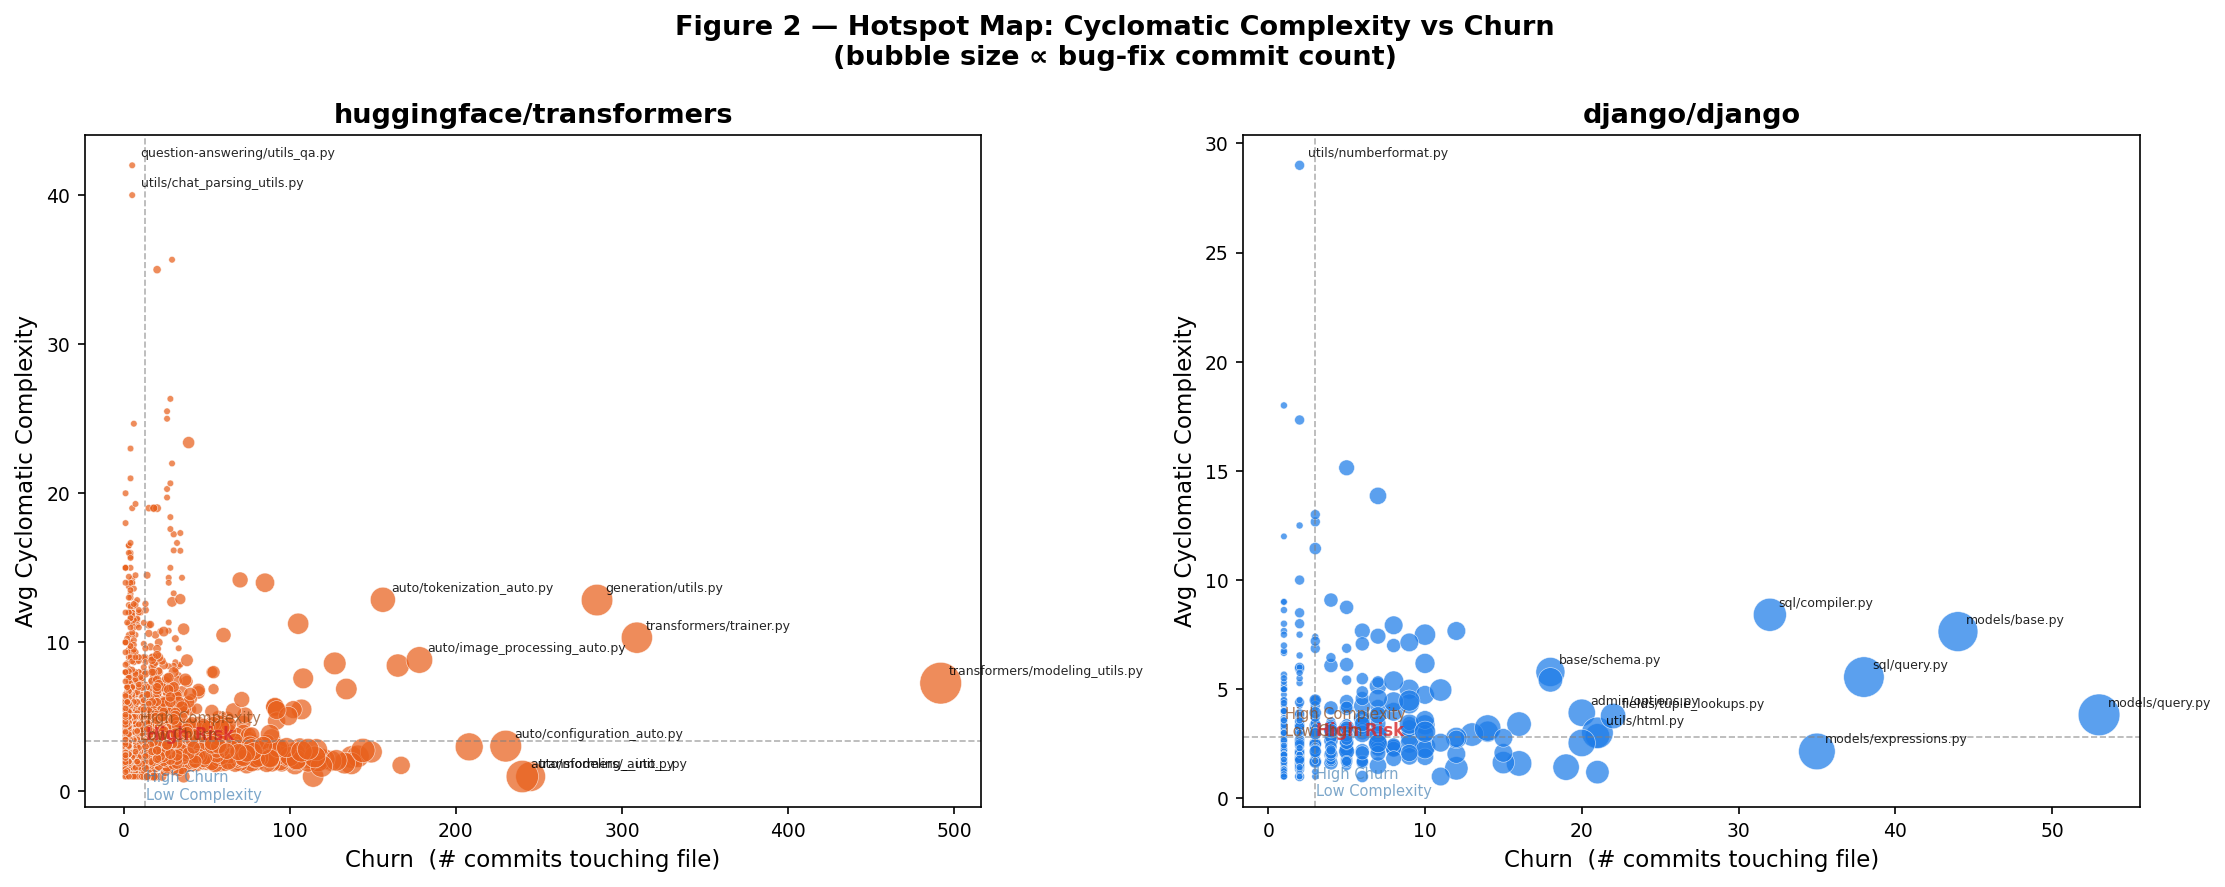
\includegraphics[width=0.95\textwidth]{plots/fig01_hotspot_scatter.png}
\caption{Hotspot scatter: cyclomatic complexity (y) vs.\ churn (x). Bubble size $\propto$ bug-fix commits. Dashed lines mark project-wide medians; the upper-right quadrant contains the highest-risk files.}
\label{fig:hotspot_scatter}
\end{figure}

Figure~\ref{fig:top_hotspots} ranks the top~15 files by composite hotspot score, and Tables~\ref{tab:top_transformers}--\ref{tab:top_django} list the top~10 with exact metric values.

\begin{figure}[!htb]
\centering
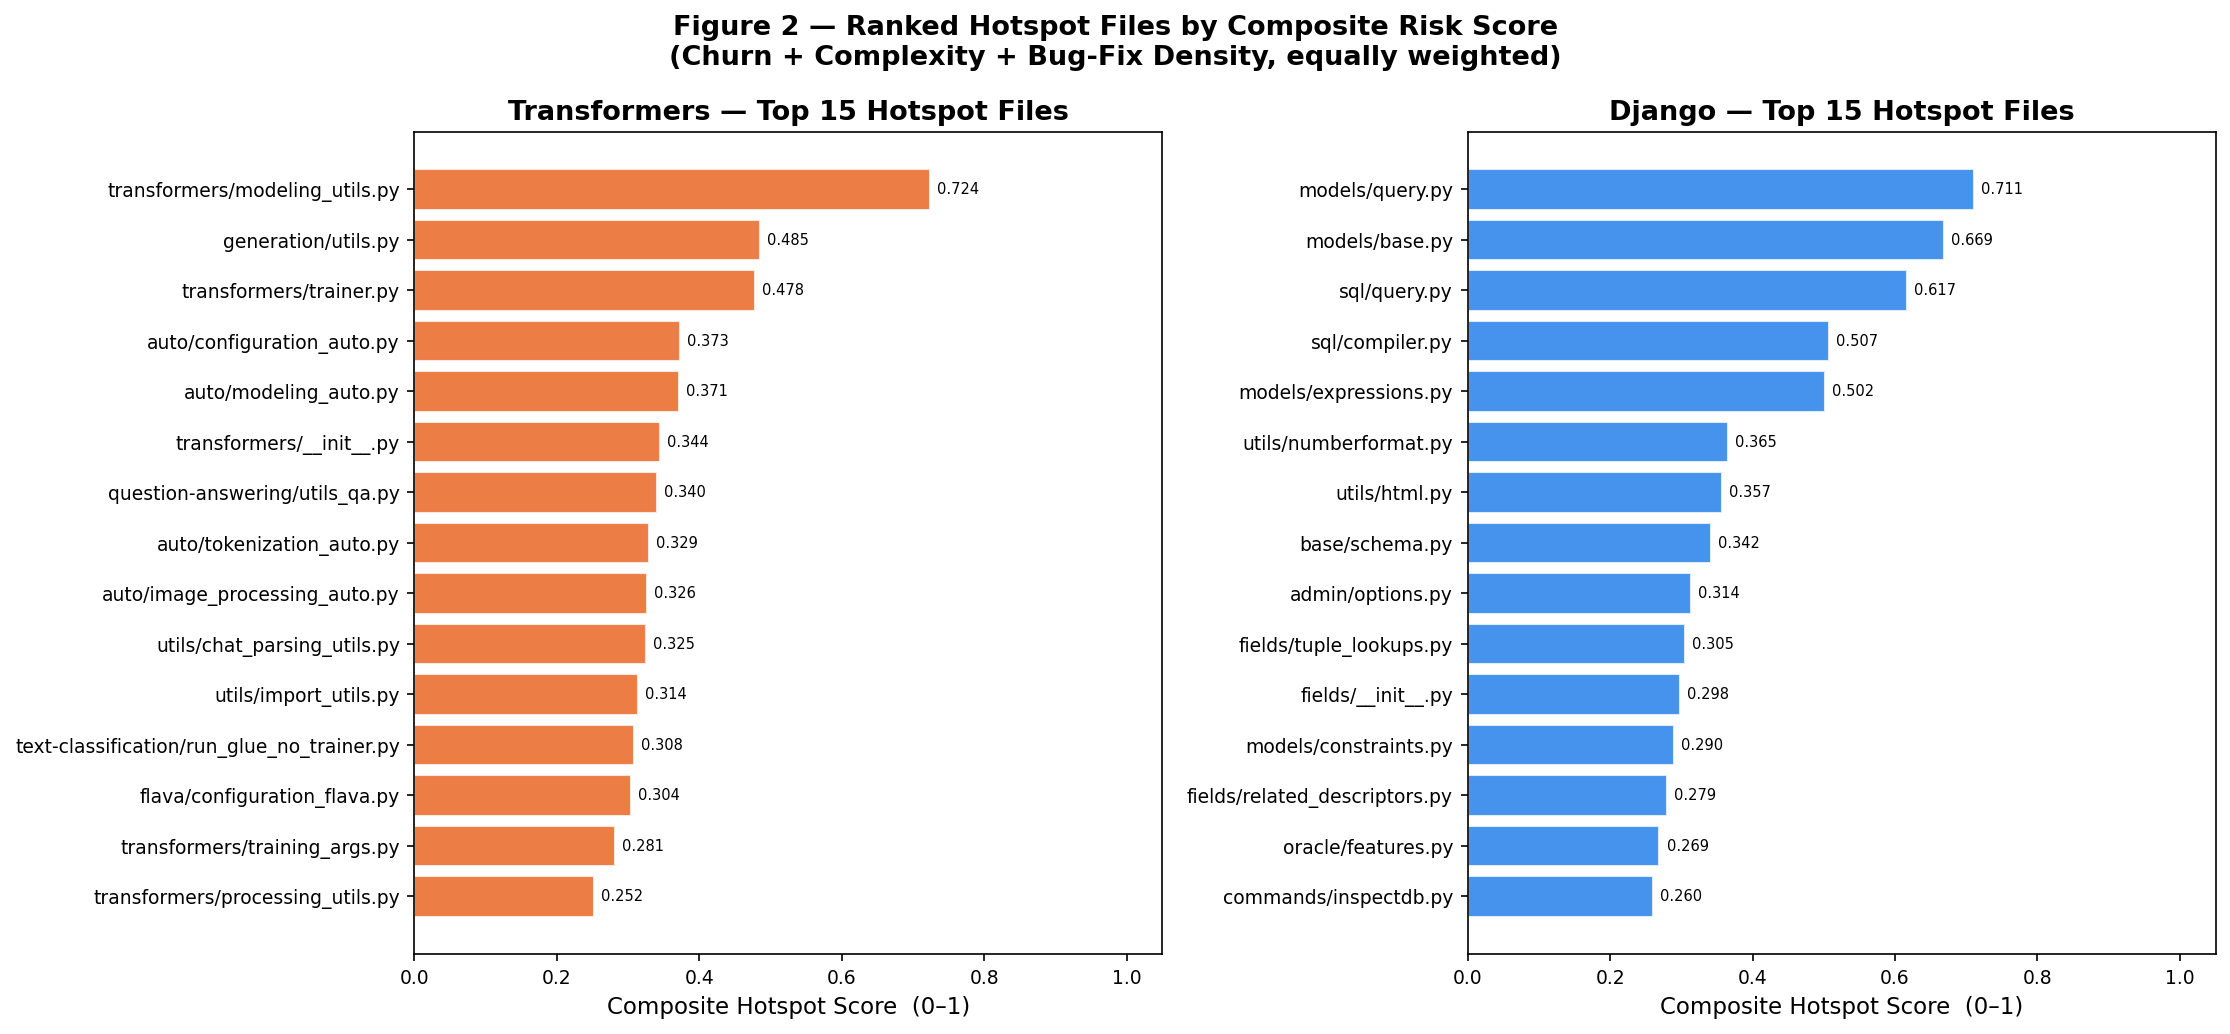
\includegraphics[width=0.95\textwidth]{plots/fig02_top_hotspots.png}
\caption{Top 15 files by composite hotspot score in each project.}
\label{fig:top_hotspots}
\end{figure}

\FloatBarrier

\begin{table}[!htb]
\centering
\footnotesize
\caption{Top 10 hotspot files --- Transformers}
\label{tab:top_transformers}
\begin{tabular}{clcccc}
\toprule
\# & File & Churn & Bug-fixes & CCN & Score \\
\midrule
1 & \texttt{modeling\_utils.py}         & 492 & 364 & 7.26  & 0.724 \\
2 & \texttt{generation/utils.py}        & 285 & 208 & 12.84 & 0.485 \\
3 & \texttt{trainer.py}                 & 309 & 204 & 10.31 & 0.478 \\
4 & \texttt{configuration\_auto.py}     & 230 & 211 & 3.04  & 0.373 \\
5 & \texttt{modeling\_auto.py}           & 240 & 219 & 1.00  & 0.371 \\
6 & \texttt{\_\_init\_\_.py}            & 245 & 186 & 1.00  & 0.344 \\
7 & \texttt{utils\_qa.py}               & 5   & 4   & 42.00 & 0.340 \\
8 & \texttt{tokenization\_auto.py}      & 156 & 132 & 12.86 & 0.329 \\
9 & \texttt{image\_processing\_auto.py} & 178 & 148 & 8.82  & 0.326 \\
10& \texttt{chat\_parsing\_utils.py}    & 5   & 5   & 40.00 & 0.325 \\
\bottomrule
\end{tabular}
\end{table}

\begin{table}[!htb]
\centering
\footnotesize
\caption{Top 10 hotspot files --- Django}
\label{tab:top_django}
\begin{tabular}{clcccc}
\toprule
\# & File & Churn & Bug-fixes & CCN & Score \\
\midrule
1 & \texttt{models/query.py}         & 53 & 35 & 3.83  & 0.711 \\
2 & \texttt{models/base.py}          & 44 & 32 & 7.64  & 0.669 \\
3 & \texttt{sql/query.py}            & 38 & 33 & 5.56  & 0.617 \\
4 & \texttt{sql/compiler.py}         & 32 & 22 & 8.41  & 0.507 \\
5 & \texttt{models/expressions.py}   & 35 & 27 & 2.15  & 0.502 \\
6 & \texttt{utils/numberformat.py}   & 2  & 2  & 29.00 & 0.365 \\
7 & \texttt{utils/html.py}           & 21 & 20 & 3.00  & 0.357 \\
8 & \texttt{base/schema.py}          & 18 & 17 & 5.79  & 0.342 \\
9 & \texttt{admin/options.py}        & 20 & 15 & 3.92  & 0.314 \\
10& \texttt{fields/tuple\_lookups.py} & 22 & 13 & 3.77  & 0.305 \\
\bottomrule
\end{tabular}
\end{table}

\textbf{Key observations.}
In \textbf{Transformers}, the top three hotspots---\texttt{modeling\_utils.py}, \texttt{generation/utils.py}, and \texttt{trainer.py}---are all core infrastructure files that every model depends on.
Their high churn stems from the library's rapid model-addition cadence: each new architecture touches these utilities.
Interestingly, files~7 and~10 (\texttt{utils\_qa.py}, \texttt{chat\_parsing\_utils.py}) have very low churn but extremely high complexity (CCN\,$>$\,40), representing a different kind of risk---latent complexity that will become dangerous the moment the files need to change.

In \textbf{Django}, the hotspot list is dominated by the ORM layer (\texttt{db/models/}, \texttt{db/sql/}).
This is consistent with the well-known difficulty of maintaining a database abstraction layer across multiple backends (SQLite, PostgreSQL, MySQL, Oracle).

\FloatBarrier
\subsection{\texorpdfstring{RQ\,2}{RQ 2}: Do Hotspots Contain More Bugs?}

\subsubsection{Correlation Analysis}

Figure~\ref{fig:corr_heatmap} shows the Pearson correlation matrix across all five raw metrics for each project.

\begin{figure}[!htb]
\centering
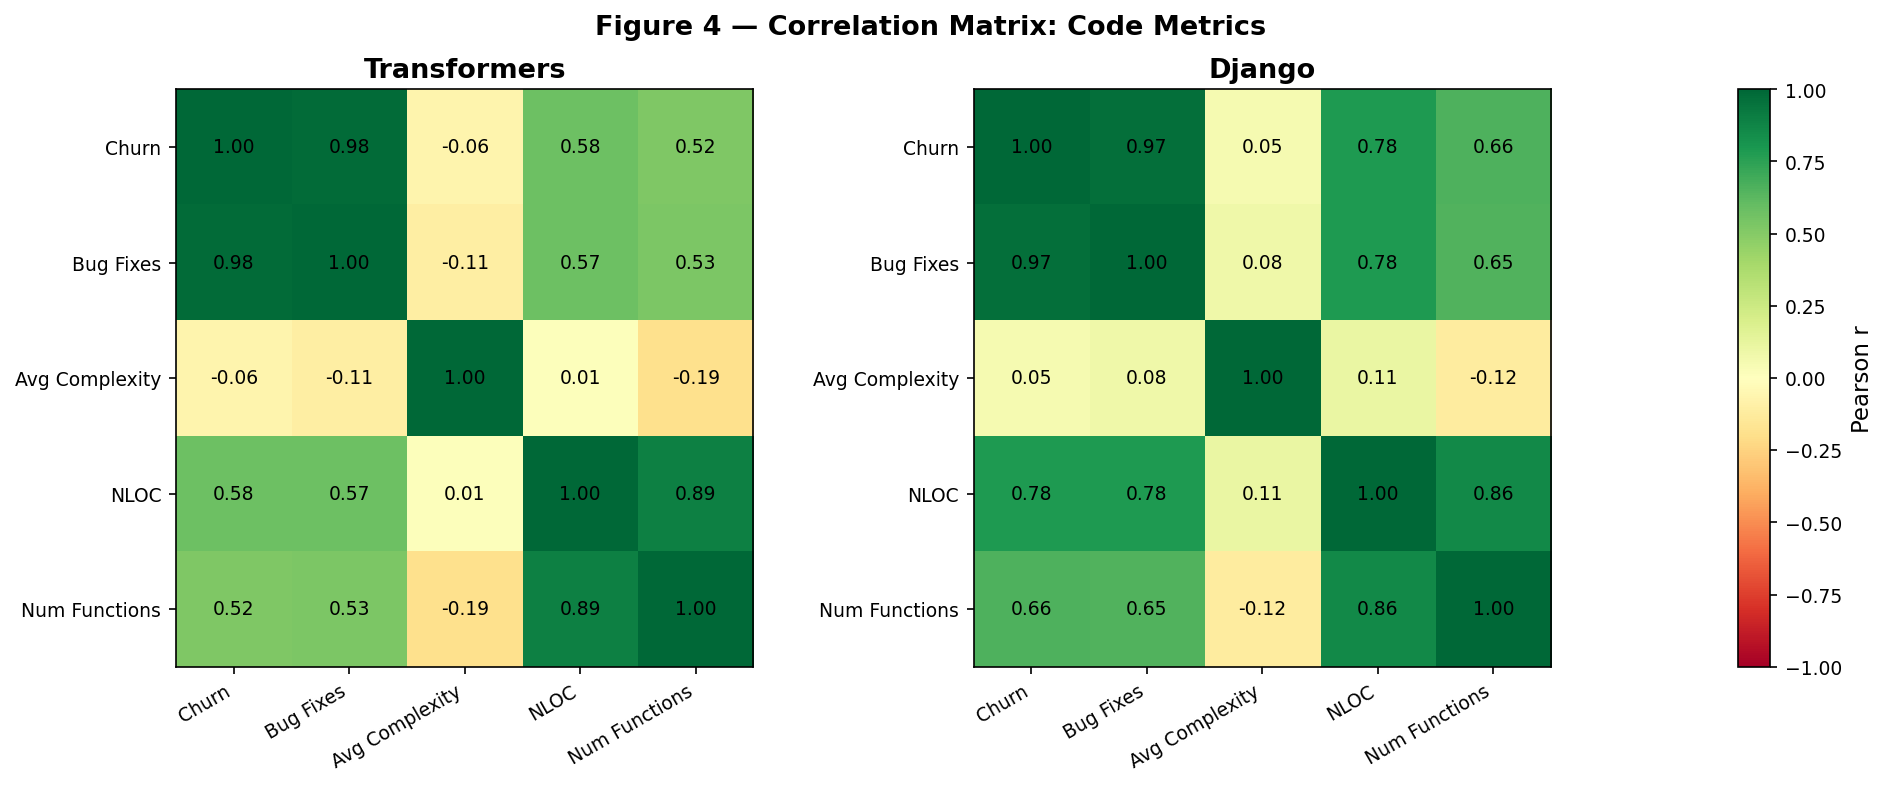
\includegraphics[width=0.92\textwidth]{plots/fig06_correlation_heatmap.png}
\caption{Pearson correlation heatmap. Churn and bug-fix count are very strongly correlated ($r > 0.96$) in both projects.}
\label{fig:corr_heatmap}
\end{figure}

\begin{table}[!htb]
\centering
\caption{Key Pearson correlations (with $p$-values)}
\label{tab:correlations}
\begin{tabular}{lcc}
\toprule
\textbf{Metric pair}                     & \textbf{Transformers}         & \textbf{Django} \\
\midrule
Churn $\leftrightarrow$ Bug-fixes        & $r=0.984\;(p\approx 0)$      & $r=0.968\;(p=7.2\times10^{-237})$ \\
Complexity $\leftrightarrow$ Bug-fixes   & $r=-0.109\;(p=4.8\times10^{-7})$ & $r=0.081\;(p=0.109)$ \\
\bottomrule
\end{tabular}
\end{table}

The churn--bug-fix correlation is near-perfect in both projects: files that change frequently are overwhelmingly more likely to be the target of corrective (bug-fix) commits.
Complexity alone shows a weak or non-significant relationship with bug-fixes, which \emph{validates the hotspot model}: it is the combination of complexity and churn that matters, not either metric in isolation~[6].

\subsubsection{Bug-Fix Ratio by Complexity Quartile}

Figure~\ref{fig:bugfix_quartile} groups files into four complexity quartiles and compares the mean bug-fix ratio in each.

\begin{figure}[!htb]
\centering
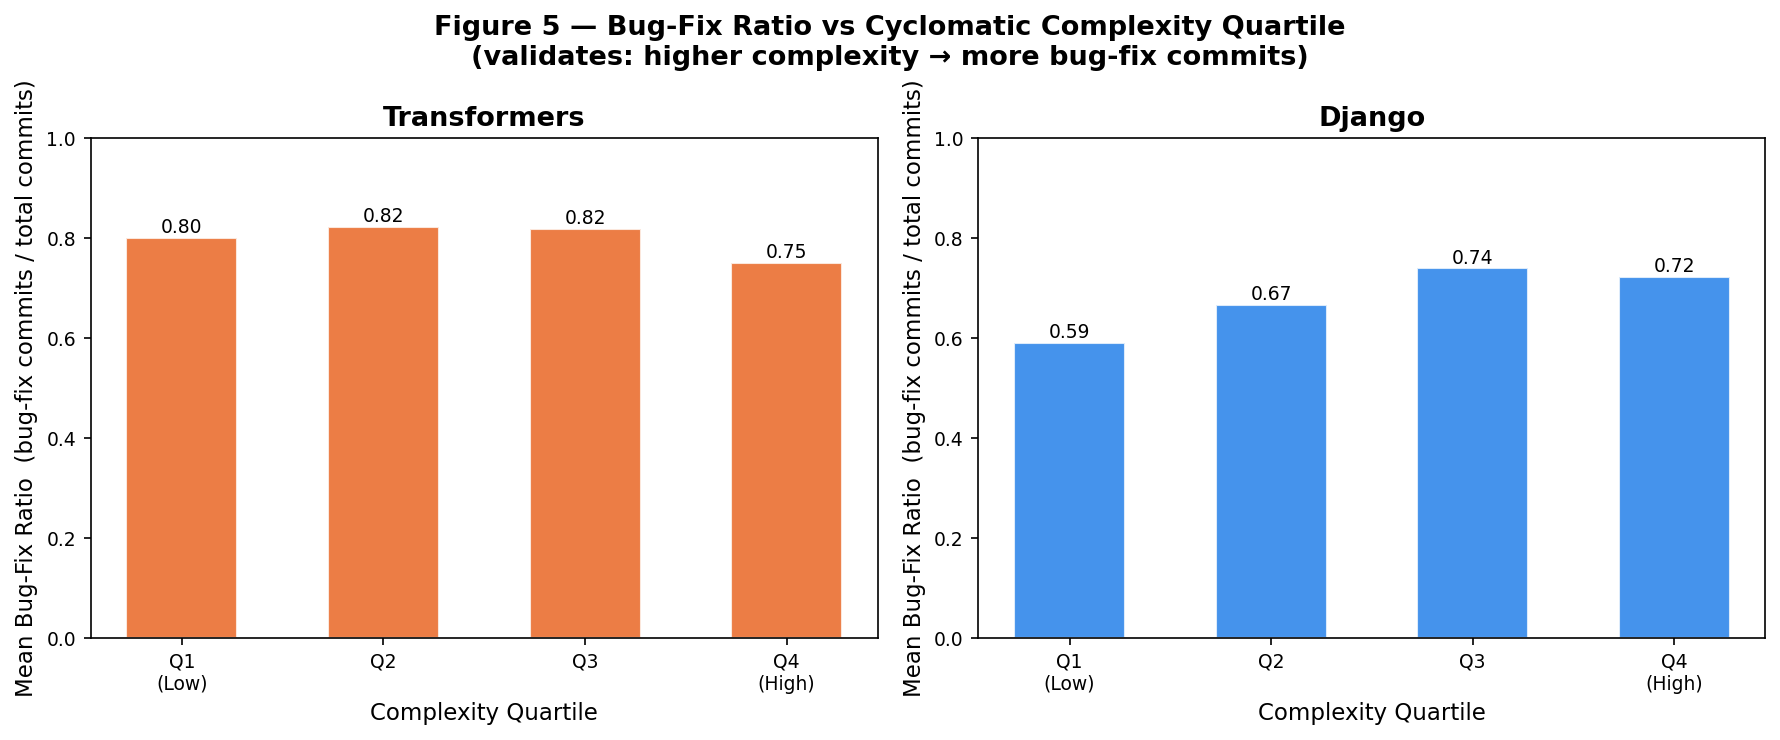
\includegraphics[width=0.92\textwidth]{plots/fig07_bugfix_ratio_by_quartile.png}
\caption{Mean bug-fix ratio (bug-fix commits / total commits) by complexity quartile. Q4 (highest complexity) consistently shows a higher proportion of corrective changes.}
\label{fig:bugfix_quartile}
\end{figure}

In both projects, the Q4 (highest-complexity) group has a meaningfully higher bug-fix ratio than Q1.
This confirms that, holding churn constant, complex code requires proportionally more corrective maintenance---supporting McCabe's original thesis~[2] and Basili and Perricone's empirical findings~[3].

\subsubsection{Top-File Overlap}

Comparing the top-10 lists by hotspot score (Tables~\ref{tab:top_transformers}--\ref{tab:top_django}) with the top-10 lists by bug-fix count alone, we find that \textbf{8 out of 10 files overlap} in Transformers and \textbf{7 out of 10 overlap} in Django.
This high overlap confirms that the composite hotspot score is capturing genuine defect-prone areas.

\FloatBarrier
\subsection{Code-Smell Indicators and Supplementary Analyses}

\subsubsection{Churn and Complexity Distributions}

Figure~\ref{fig:churn_dist} reveals a heavy-tailed (near power-law) distribution of churn: a small fraction of files absorbs the vast majority of changes, consistent with the Pareto principle widely observed in software evolution research~[5].

\begin{figure}[!htb]
\centering
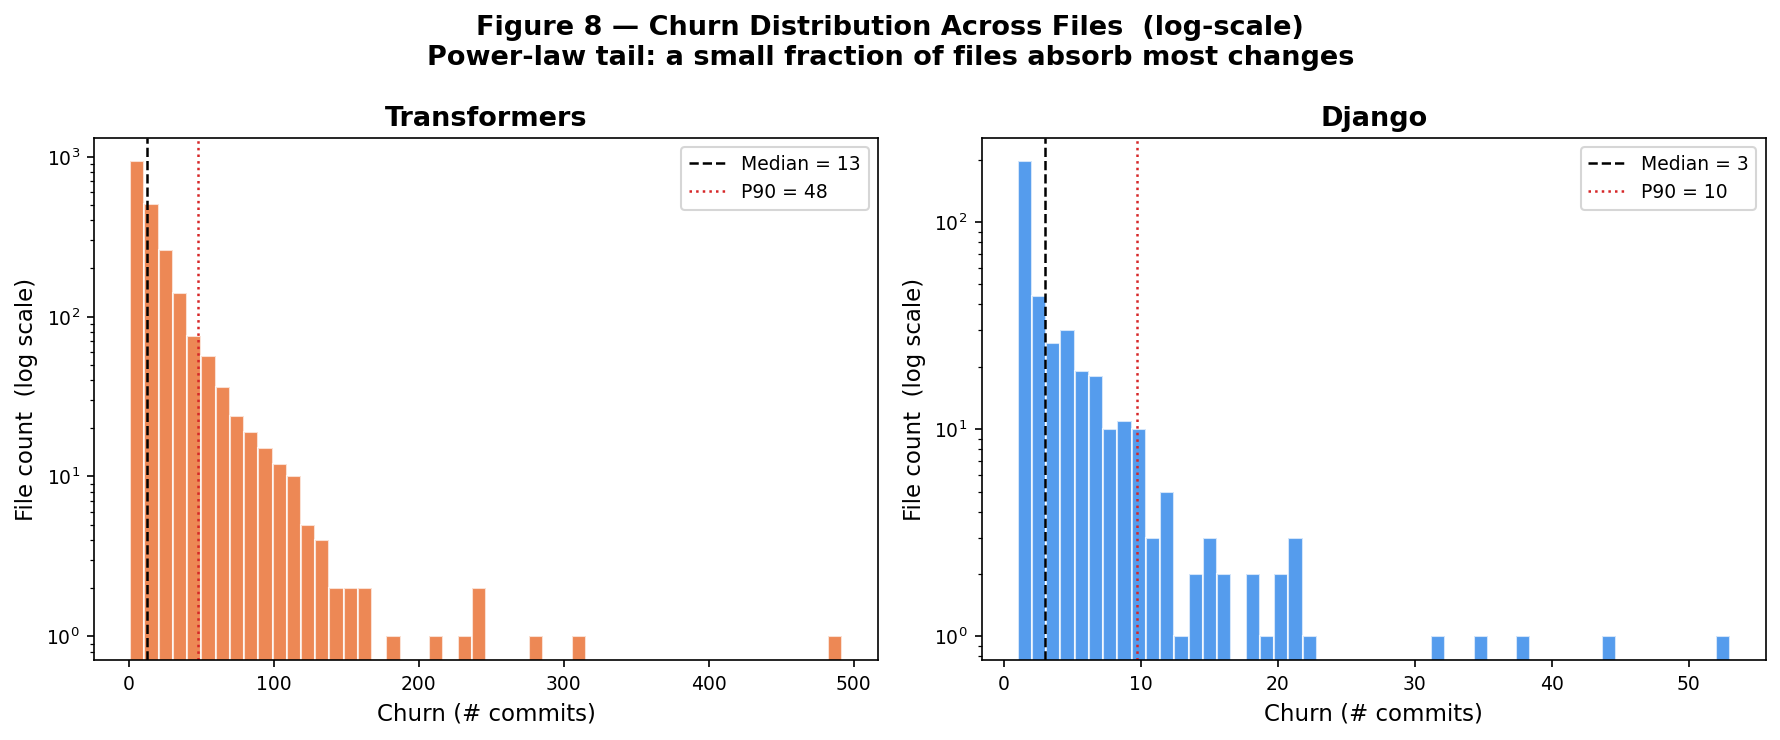
\includegraphics[width=0.92\textwidth]{plots/fig08_churn_distribution.png}
\caption{Churn distribution (log-scale y-axis). Dashed lines: median and 90th percentile.}
\label{fig:churn_dist}
\end{figure}

Figure~\ref{fig:complexity_dist} shows that most files have low complexity (CCN\,$<$\,5), but a notable tail exceeds the McCabe thresholds of 10 (moderate risk) and 20 (high risk).

\begin{figure}[!htb]
\centering
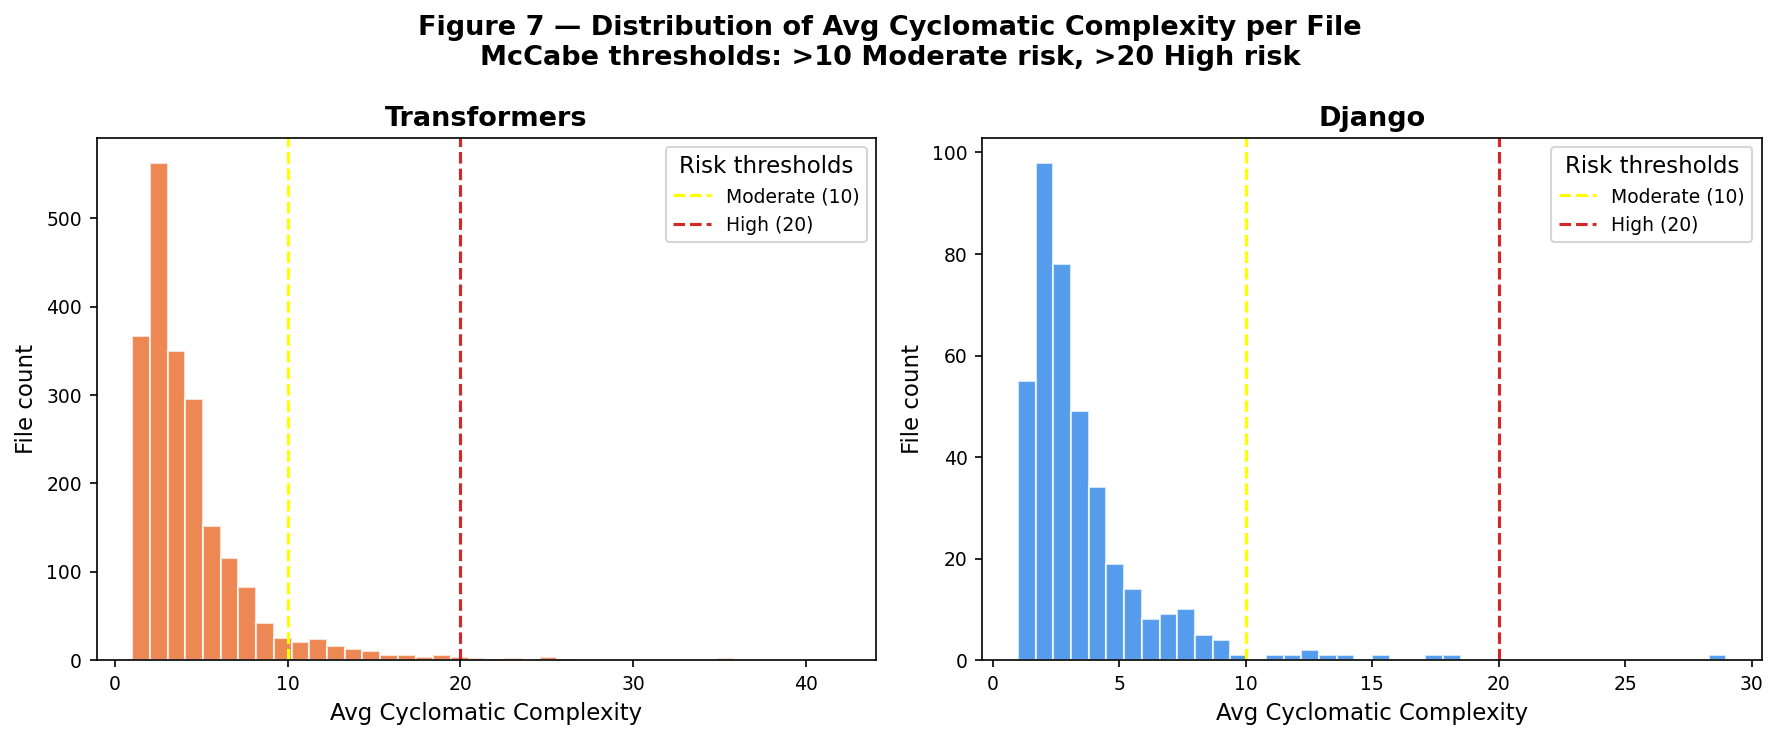
\includegraphics[width=0.92\textwidth]{plots/fig09_complexity_distribution.png}
\caption{Distribution of average cyclomatic complexity. Dashed lines: McCabe risk thresholds at 10 and 20.}
\label{fig:complexity_dist}
\end{figure}

\FloatBarrier
\subsubsection{File Size vs.\ Complexity (God Module Detection)}

Large files with many functions and elevated complexity are symptomatic of the \emph{God Module} code smell~[9].
Figure~\ref{fig:nloc_complexity} plots NLOC against average CCN (bubble size $\propto$ churn).

\begin{figure}[!htb]
\centering
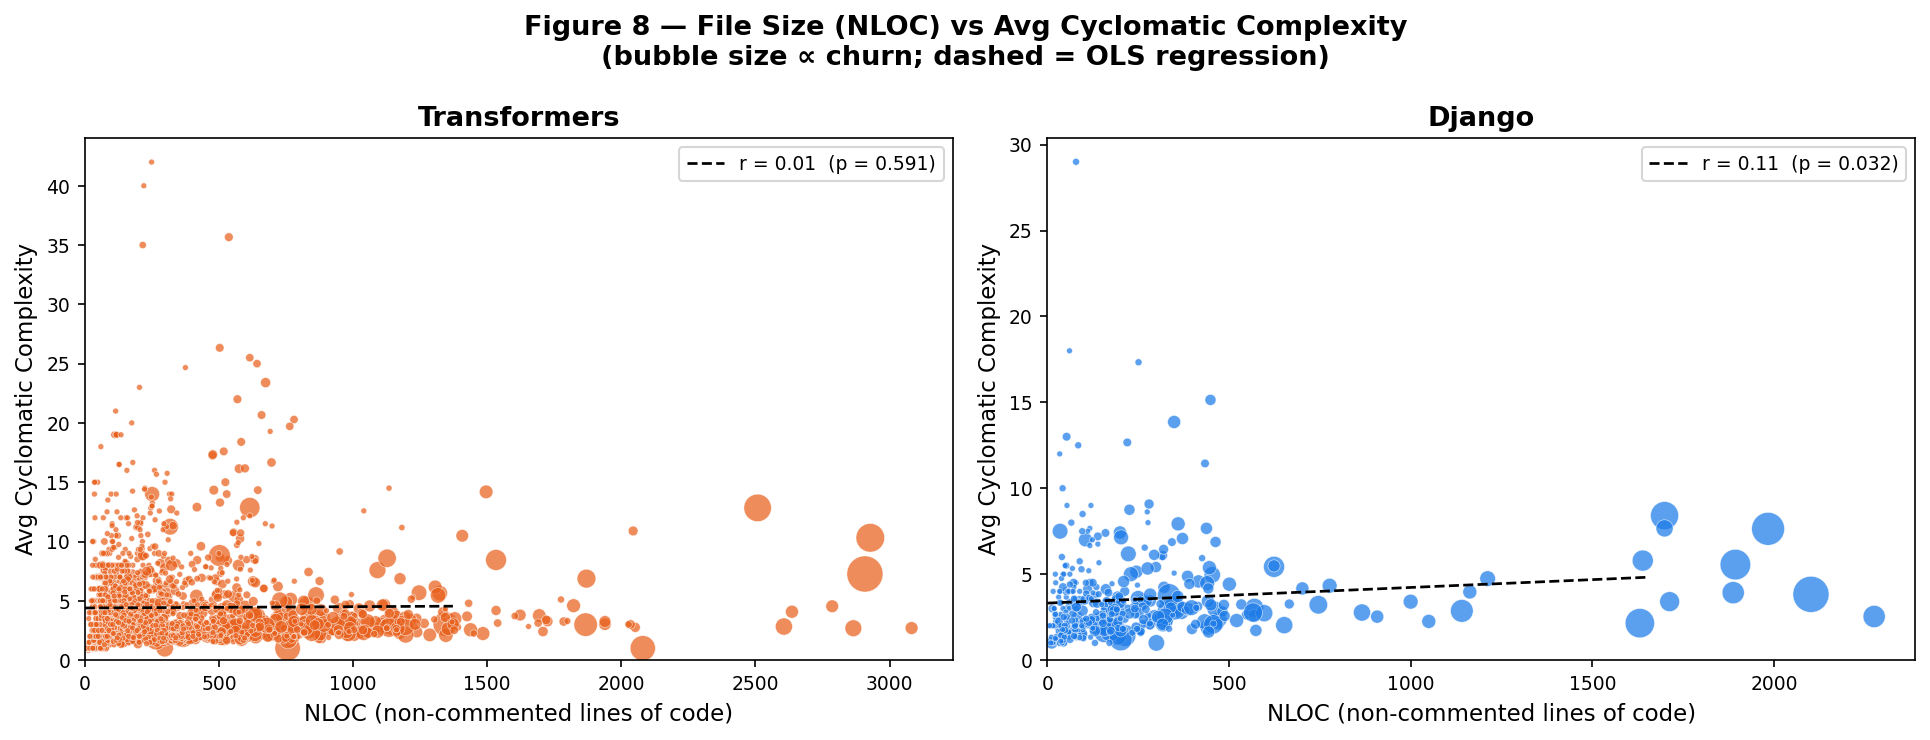
\includegraphics[width=0.92\textwidth]{plots/fig10_nloc_vs_complexity.png}
\caption{NLOC vs.\ average complexity (bubble size $\propto$ churn; dashed = OLS regression).}
\label{fig:nloc_complexity}
\end{figure}

Files with NLOC\,$>$\,1000 and elevated complexity---such as \texttt{modeling\_utils.py} (2\,908~NLOC) and \texttt{trainer.py} (2\,928~NLOC) in Transformers---are prime candidates for module decomposition.

\subsubsection{Lines Added vs.\ Lines Deleted}

Figure~\ref{fig:lines_added_deleted} distinguishes growing files (below the 45\textdegree{} diagonal) from shrinking files (above it), helping to identify files undergoing net growth (feature creep) versus net contraction (refactoring).

\begin{figure}[!htb]
\centering
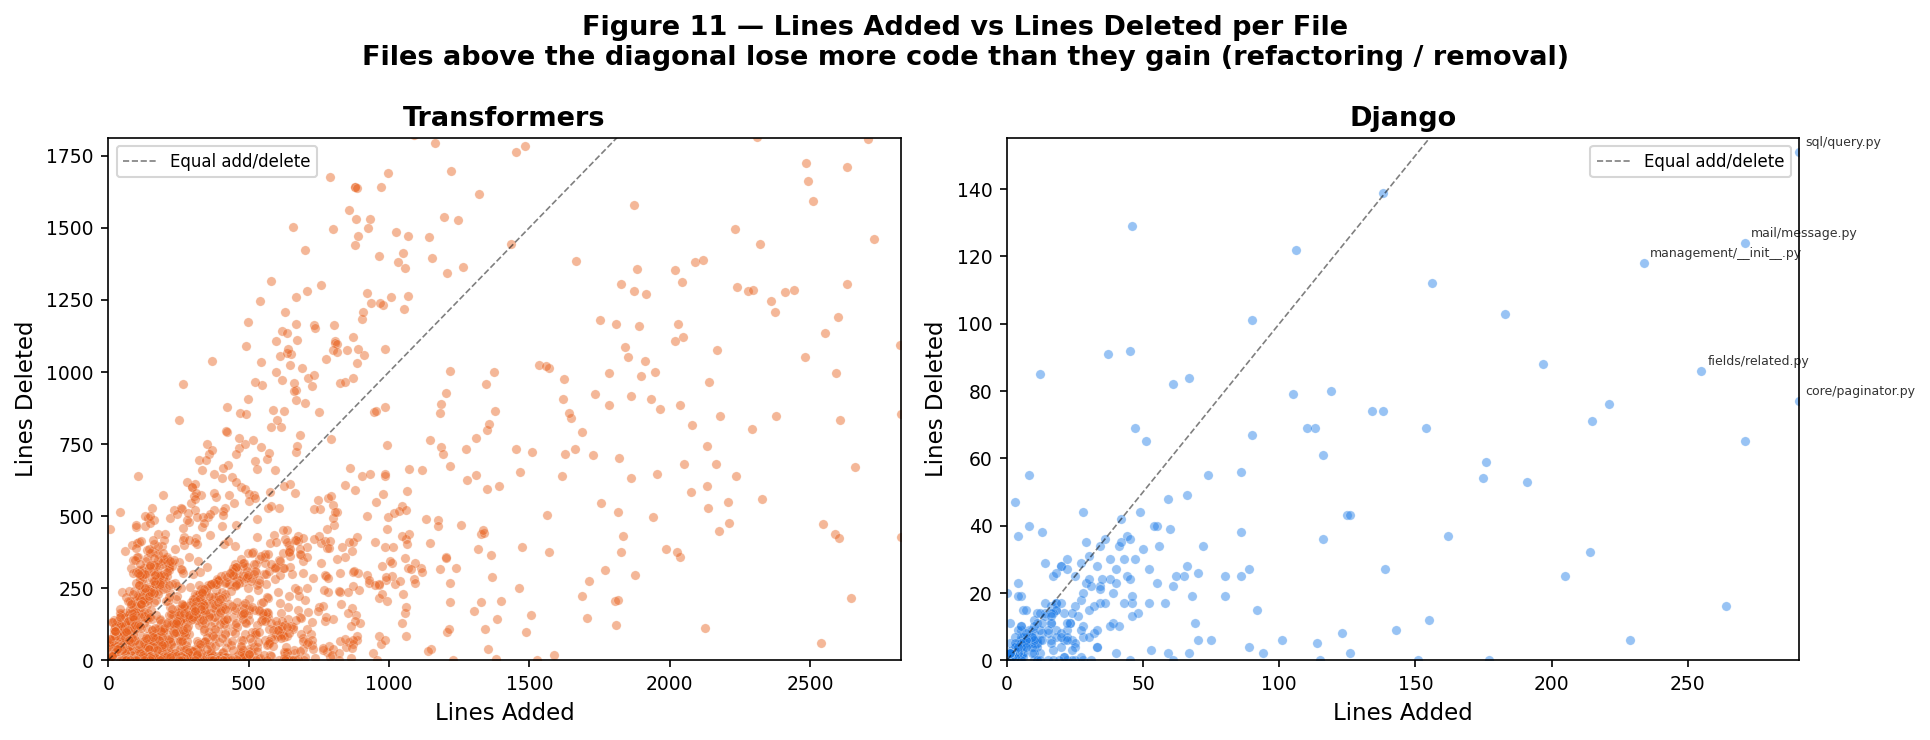
\includegraphics[width=0.92\textwidth]{plots/fig11_lines_added_deleted.png}
\caption{Lines added vs.\ lines deleted. The 45\textdegree{} line denotes equal churn in both directions.}
\label{fig:lines_added_deleted}
\end{figure}

\FloatBarrier
\subsection{\texorpdfstring{RQ\,3}{RQ 3}: Prioritised Remediation Plan}

Figure~\ref{fig:remediation_matrix} classifies the top~20 hotspot files into the four-quadrant remediation model.
Tables~\ref{tab:plan_transformers} and~\ref{tab:plan_django} present the prioritised remediation plans with file-specific recommended actions.

\begin{figure}[!htb]
\centering
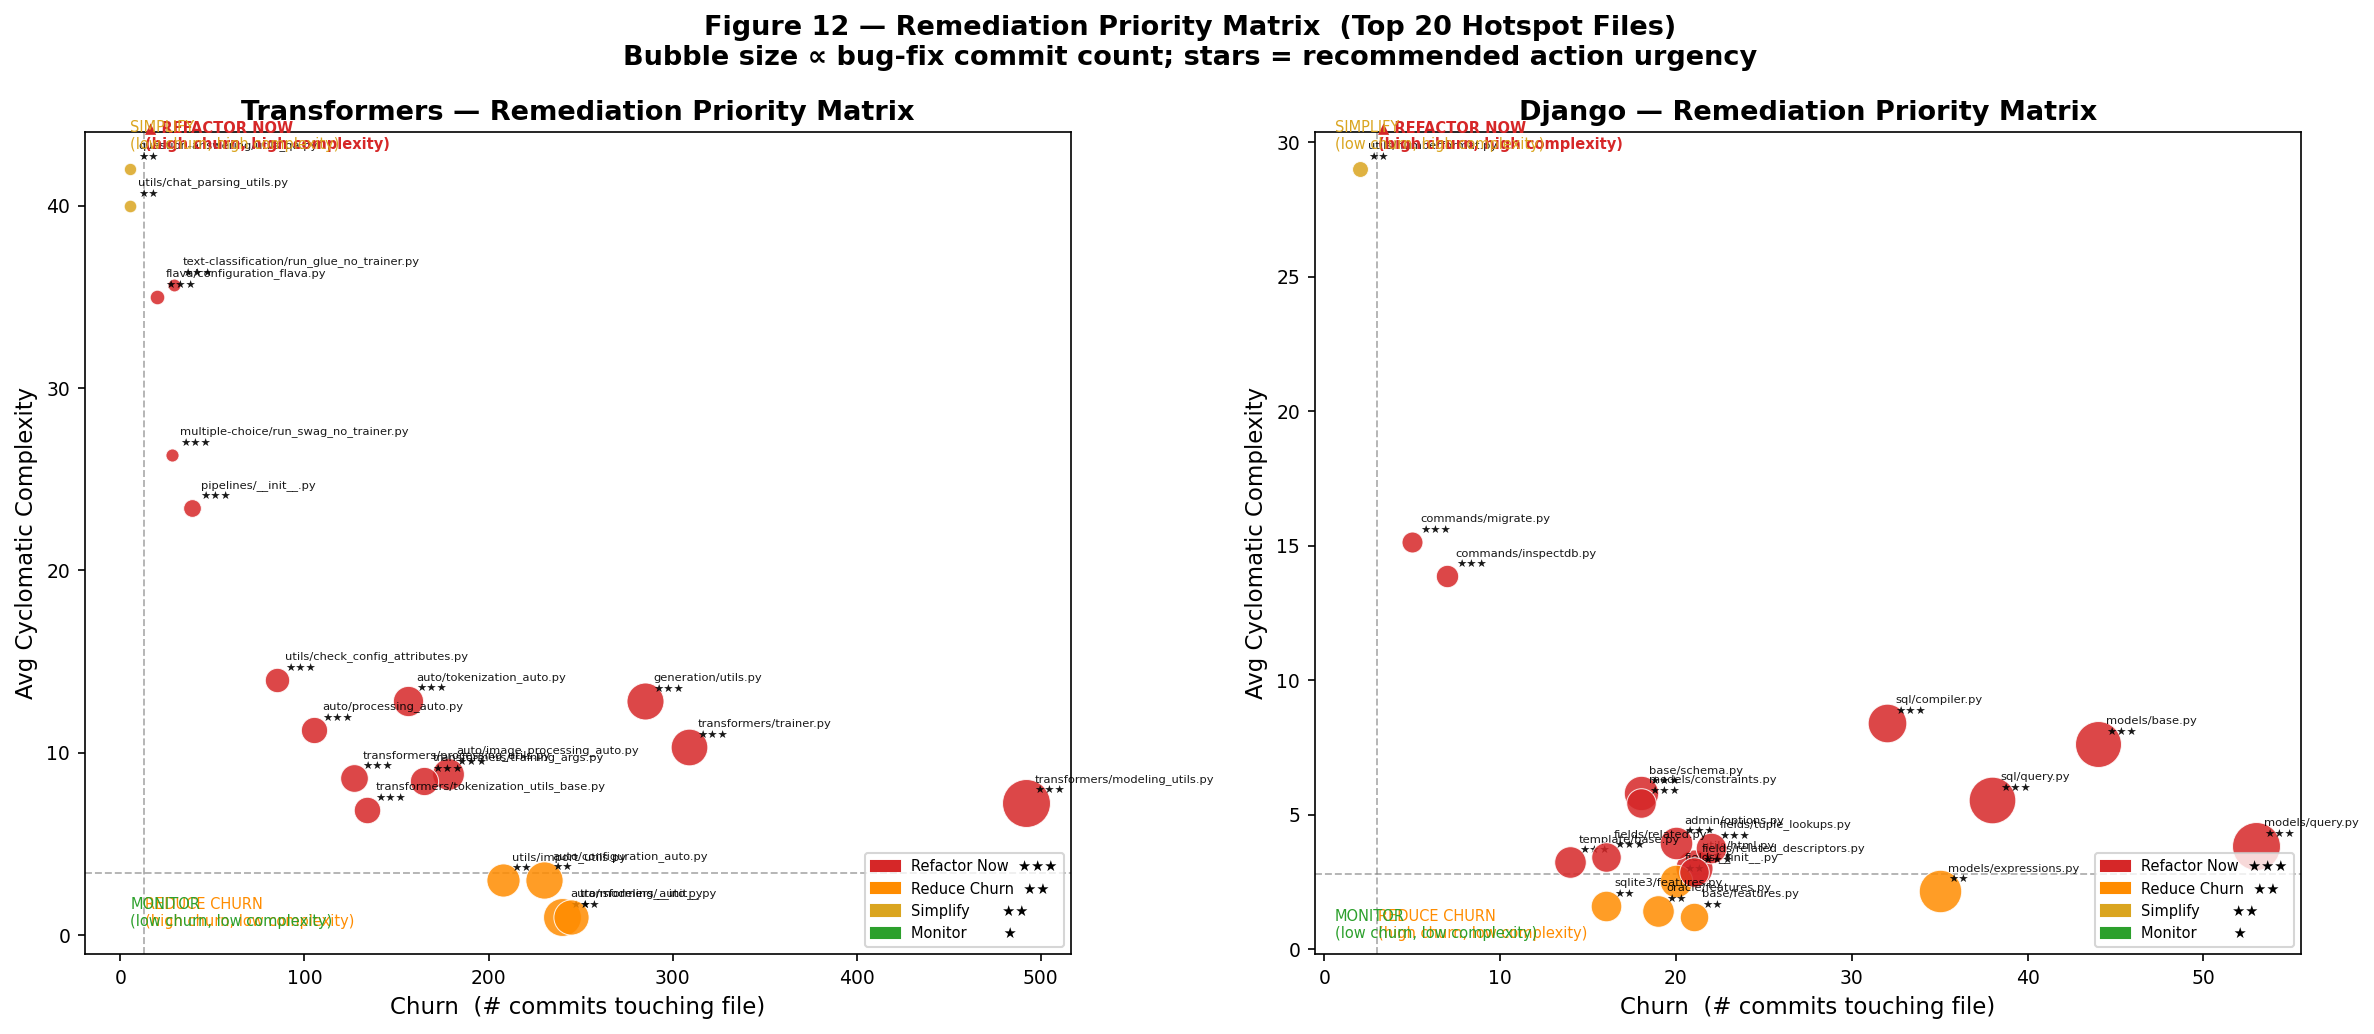
\includegraphics[width=0.95\textwidth]{plots/fig12_remediation_matrix.png}
\caption{Remediation priority matrix (top 20 files). Bubble size $\propto$ bug-fix count; star rating = action urgency.}
\label{fig:remediation_matrix}
\end{figure}

\begin{table}[!htb]
\centering
\footnotesize
\caption{Prioritised remediation plan --- Transformers (top 10)}
\label{tab:plan_transformers}
\begin{tabular}{cl c c c p{5cm}}
\toprule
\textbf{\#} & \textbf{File} & \textbf{CCN} & \textbf{Churn} & \textbf{Bugs} & \textbf{Recommended Action} \\
\midrule
1 & \texttt{modeling\_utils.py}       & 7.26  & 492 & 364 & Split into sub-modules (loading, saving, device management). Add integration tests. \\
2 & \texttt{generation/utils.py}      & 12.84 & 285 & 208 & Extract beam search, sampling, and stopping criteria into separate classes. \\
3 & \texttt{trainer.py}               & 10.31 & 309 & 204 & Decompose into training loop, evaluation, and callback manager. \\
4 & \texttt{utils\_qa.py}             & 42.00 & 5   & 4   & Refactor monolithic post-processing (CCN=42 is critically high). \\
5 & \texttt{chat\_parsing\_utils.py}  & 40.00 & 5   & 5   & Break monolithic parsing functions into smaller, testable units. \\
6 & \texttt{tokenization\_auto.py}    & 12.86 & 156 & 132 & Add regression tests; stabilise auto-resolution logic. \\
7 & \texttt{configuration\_auto.py}   & 3.04  & 230 & 211 & Freeze interface; add automated config-validation tests. \\
8 & \texttt{modeling\_auto.py}        & 1.00  & 240 & 219 & Improve code-generation tooling to reduce manual mapping edits. \\
9 & \texttt{image\_proc\_auto.py}     & 8.82  & 178 & 148 & Increase test coverage; stabilise preprocessing API. \\
10& \texttt{\_\_init\_\_.py}          & 1.00  & 245 & 186 & Adopt lazy-import pattern to reduce churn from model additions. \\
\bottomrule
\end{tabular}
\end{table}

\begin{table}[!htb]
\centering
\footnotesize
\caption{Prioritised remediation plan --- Django (top 10)}
\label{tab:plan_django}
\begin{tabular}{cl c c c p{5cm}}
\toprule
\textbf{\#} & \textbf{File} & \textbf{CCN} & \textbf{Churn} & \textbf{Bugs} & \textbf{Recommended Action} \\
\midrule
1 & \texttt{models/query.py}       & 3.83 & 53 & 35 & Add targeted unit tests; refactor long QuerySet method chains. \\
2 & \texttt{models/base.py}        & 7.64 & 44 & 32 & Extract metaclass logic into separate mixins. \\
3 & \texttt{sql/query.py}          & 5.56 & 38 & 33 & Add edge-case tests for complex SQL-construction paths. \\
4 & \texttt{sql/compiler.py}       & 8.41 & 32 & 22 & Extract dialect-specific compilation into backend modules. \\
5 & \texttt{models/expressions.py} & 2.15 & 35 & 27 & Stabilise expression API; improve backward-compat guards. \\
6 & \texttt{utils/numberformat.py}  & 29.00& 2  & 2  & Decompose single monolithic function (CCN=29). \\
7 & \texttt{utils/html.py}         & 3.00 & 21 & 20 & Bug-fix ratio 95\%; add fuzz tests for HTML sanitisation. \\
8 & \texttt{base/schema.py}        & 5.79 & 18 & 17 & Improve test coverage for cross-database schema migration. \\
9 & \texttt{admin/options.py}      & 3.92 & 20 & 15 & Decompose by feature area (list, detail, inline). \\
10& \texttt{tuple\_lookups.py}     & 3.77 & 22 & 13 & Add regression tests; moderate risk, monitor going forward. \\
\bottomrule
\end{tabular}
\end{table}

\FloatBarrier
\subsection{Cross-Project Comparison}

\begin{table}[!htb]
\centering
\caption{Cross-project comparison}
\label{tab:comparison}
\begin{tabular}{lrr}
\toprule
\textbf{Metric}                         & \textbf{Transformers} & \textbf{Django} \\
\midrule
Files in final analysis                  & 2\,112                & 394             \\
$r$(churn, bug-fixes)                    & 0.984                 & 0.968           \\
$r$(complexity, bug-fixes)               & $-0.109$              & 0.081           \\
Top-file churn                           & 492                   & 53              \\
Top-file bug-fixes                       & 364                   & 35              \\
Max average CCN                          & 42.0                  & 29.0            \\
\bottomrule
\end{tabular}
\end{table}

Transformers' absolute churn is roughly $10\times$ higher than Django's, consistent with its much faster release cadence.
Despite this scale difference, the churn--bug-fix correlation is remarkably similar ($r \geq 0.96$), confirming that the hotspot technique generalises across project types.
The hotspot concentration differs architecturally: in Transformers the risk centres on core utility/auto-mapping files, whereas in Django it concentrates in the ORM subsystem.

% ══════════════════════════════════════════════════════════════════════════════
\section{Threats to Validity / Limitations}
\label{sec:threats}

\paragraph{Construct validity.}
The bug-fix keyword heuristic is an imperfect proxy for true defect counts.
Mockus and Votta~[10] estimate its precision at roughly 60--70\%.
Some bug-fix commits may omit these keywords, and some non-bug commits (e.g.\ ``fix typo in docstring'') may be falsely classified.
A more robust approach would link commits to issue trackers, but this was beyond the scope of a lab-scale study.

\paragraph{Internal validity.}
The composite score uses equal weights for churn, complexity, and bug-fixes.
In practice, one metric may be a stronger predictor than the others for a given project; learning optimal weights from labelled defect data~[4] could improve ranking accuracy.
Additionally, the two-year history window may miss older, deeply embedded debt.

\paragraph{External validity.}
The study examines only two Python repositories.
The hotspot technique is language-agnostic in principle, but the specific metric thresholds (e.g.\ McCabe's CCN=10 boundary) were calibrated on C/Fortran code~[2] and may not transfer directly to Python, where language idioms like list comprehensions can compress control flow.

\paragraph{Confounding factors.}
Churn is partly a function of module centrality---core files are changed more often simply because they are imported by more modules.
Separating ``architectural churn'' from ``defect-induced churn'' would require finer-grained commit classification, which we leave to future work.

\paragraph{Reproducibility.}
All scripts and data files are included in the project repository, allowing full reproduction.
However, rerunning the history-mining step at a later date will produce different results as new commits accumulate.

% ══════════════════════════════════════════════════════════════════════════════
\section{Expected Outcome}
\label{sec:expected}

Before undertaking the analysis, we formulated three expected outcomes based on the literature:

\begin{enumerate}[leftmargin=2em]
  \item \textbf{A small number of files will dominate the risk landscape.}
        Nagappan and Ball~[4] and Tornhill~[6] predict that defects follow a Pareto distribution.
        \emph{Result: confirmed.}
        In Transformers, the top~3 files (0.14\% of the codebase) account for 776 of 3\,474 total bug-fix-related file touches ($\approx$22\%).
        In Django, the top~3 files (0.76\%) account for 100 of 430 ($\approx$23\%).

  \item \textbf{Churn will be a stronger predictor of bugs than complexity.}
        Prior work~[4,\,5] consistently finds churn superior to static metrics.
        \emph{Result: confirmed.}
        Churn correlates with bug-fixes at $r > 0.96$ in both projects, while complexity correlates at $|r| < 0.12$.

  \item \textbf{The hotspot model will surface architecturally central modules.}
        Kazman et al.~[12] showed that technical debt concentrates in architectural ``hubs.''
        \emph{Result: confirmed.}
        The top hotspots are precisely the central infrastructure files: \texttt{modeling\_utils.py} in Transformers, \texttt{models/query.py} in Django.
\end{enumerate}

All three expectations are borne out by the data, lending confidence to the hotspot identification approach and confirming its suitability as a practical technical-debt management tool for real-world software teams.

% ══════════════════════════════════════════════════════════════════════════════
\section*{References}
\addcontentsline{toc}{section}{References}

\begin{enumerate}[leftmargin=2em, label={[\arabic*]}]
  \item W.\ Cunningham, ``The WyCash Portfolio Management System,'' \emph{OOPSLA Experience Report}, 1992.
  \item T.\ J.\ McCabe, ``A Complexity Measure,'' \emph{IEEE Trans.\ Software Engineering}, vol.\ SE-2, no.\ 4, pp.\ 308--320, 1976.
  \item V.\ R.\ Basili and B.\ T.\ Perricone, ``Software Errors and Complexity: An Empirical Investigation,'' \emph{Comm.\ ACM}, vol.\ 27, no.\ 1, pp.\ 42--52, 1984.
  \item N.\ Nagappan and T.\ Ball, ``Use of Relative Code Churn Measures to Predict System Defect Density,'' \emph{Proc.\ 27th ICSE}, pp.\ 284--292, 2005.
  \item A.\ E.\ Hassan, ``Predicting Faults Using the Complexity of Code Changes,'' \emph{Proc.\ 31st ICSE}, pp.\ 78--88, 2009.
  \item A.\ Tornhill, \emph{Your Code as a Crime Scene}, Pragmatic Bookshelf, 2015.
  \item P.\ Kruchten, R.\ L.\ Nord, and I.\ Ozkaya, ``Technical Debt: From Metaphor to Theory and Practice,'' \emph{IEEE Software}, vol.\ 29, no.\ 6, pp.\ 18--21, 2012.
  \item M.\ Fowler, ``Technical Debt,'' \url{https://martinfowler.com/bliki/TechnicalDebt.html}, 2009.
  \item M.\ Fowler and K.\ Beck, \emph{Refactoring: Improving the Design of Existing Code}, Addison-Wesley, 1999.
  \item A.\ Mockus and L.\ G.\ Votta, ``Identifying Reasons for Software Changes Using Historic Databases,'' \emph{Proc.\ ICSM}, pp.\ 120--130, 2000.
  \item G.\ Spadini, M.\ Aniche, and A.\ Bacchelli, ``PyDriller: Python Framework for Mining Software Repositories,'' \emph{Proc.\ ESEC/FSE}, pp.\ 908--911, 2018.
  \item R.\ Kazman, Y.\ Cai, R.\ Mo, Q.\ Feng, L.\ Xiao, S.\ Haziyev, V.\ Fedak, and A.\ Shapochka, ``A Case Study in Locating the Architectural Roots of Technical Debt,'' \emph{Proc.\ 37th ICSE}, vol.\ 2, pp.\ 179--188, 2015.
  \item T.\ Yin, ``Lizard: A Modern Code Complexity Analyzer,'' \url{https://github.com/terryyin/lizard}, 2023.
\end{enumerate}

\end{document}
